In this chapter, results obtained by feature selection and modeling are shown with respect for each different period, resolution and target variable. 

\section{Case of Study}
This case of study aims to discover the main factors which affects mostly the target variable chosen. In order to examine the behavior of each variable in a data set over time, several grid data are collected, each one with different resolution, period and configuration:
\subsection{Data sets description}
\subsubsection{Period}  
Data collected are dated 2021 because are the most recent and, with respect 2020, the ones not particularly affecting by emission reduction caused by lockdown for COVID-19 pandemic\cite{bontempi2022analysis}. In this case of study grid data are chosen by considering the effect of intensive agriculture, with these particular condition:
    \begin{itemize}
        \item In order to have right condition for farming, in the period chosen the terrain shouldn't be frozen (Temperature > 0°C). So I selected data coming from spring, summer and autumn period (discarding winter);
        \item For better highlighting the effect of intense agriculture with the usage of fertilizer and pesticides, which are the main pollution emission factors, weeks preceding a rain period are selected;
\end{itemize}
In this way, several grid data are chosen from 5 different weeks:
\begin{itemize}
    \item 24 March - 31 March 2021;
    \item 18 April - 25 April 2021;
    \item 17 July - 24 July 2021;
    \item 3 September - 10 September 2021;
    \item 7 October - 14 October 2021
\end{itemize}
\subsubsection{Resolutions}
0.1° ($\sim$ 10km) and 0.01° ($\sim$ 1km) resolutions are selected for the grid data. For increasing the number of observation provided by the limited ARPA stations in Lombardy a k-nearest neighbors algorithm is applied to adding the buffer of values (with k respectively equal to 10 and 30 for each resolution). Then, the value added are computed using the RBF interpolation (as already explained in the \hyperref[sec:Data cleaning]{Data Cleaning section}.

\subsubsection{Target Variables}
PM25 and ammonia (NH3) provided by ARPA sensors are the one chosen as target variables. I chose them because are strictly related between them and are the most related to intense farming pollution.

\subsubsection{Mountains}
Another important parameter configuration used is to filter or not the cell covered by mountains or not (climate zone = 1/2/3 of Alpes and Prealpes). In this way the test run can take in consideration or not only urban and land areas, which are more affected by air pollution phenomena.


\subsubsection{Feature Selection}
After the preprocessing phase, I use 2 different configuration for training ML models:
\begin{itemize}
    \item Using the set of variables selected for each different period;
    \item Using a general set of variables. This was computed by averaging the feature selected for each different period with Borda Count another time;
\end{itemize}


-data
-motivazioni
-risoluzioni
-parametri test
\pagebreak
\section{FS Results}
\subsection{Target variable = 'pm25\_st' \& resolution = 0.01°}
\centering
\subsubsection{Including mountains}
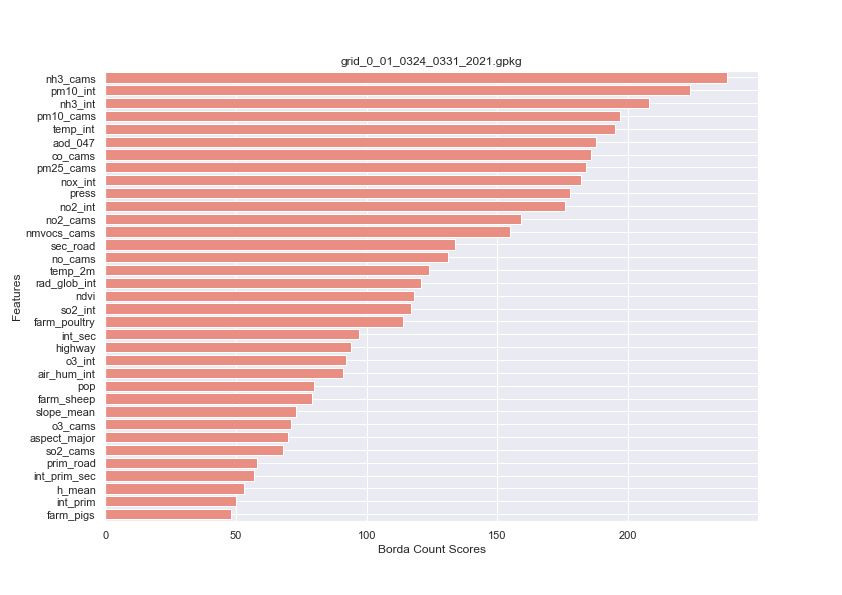
\includegraphics[width=0.9\textwidth]{images/fs_results/pm25/001/montains/grid_0_01_0324_0331_2021.png}
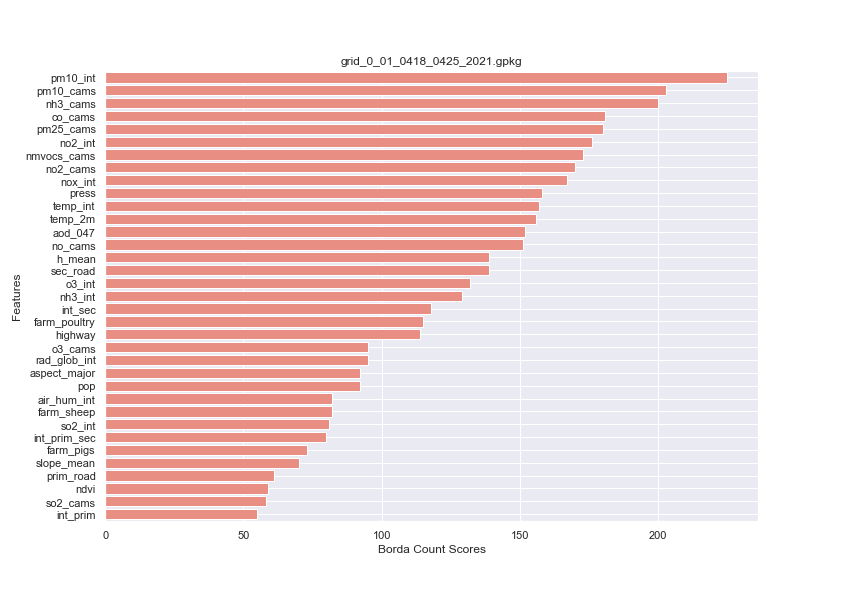
\includegraphics[width=0.9\textwidth]{images/fs_results/pm25/001/montains/grid_0_01_0418_0425_2021.png}
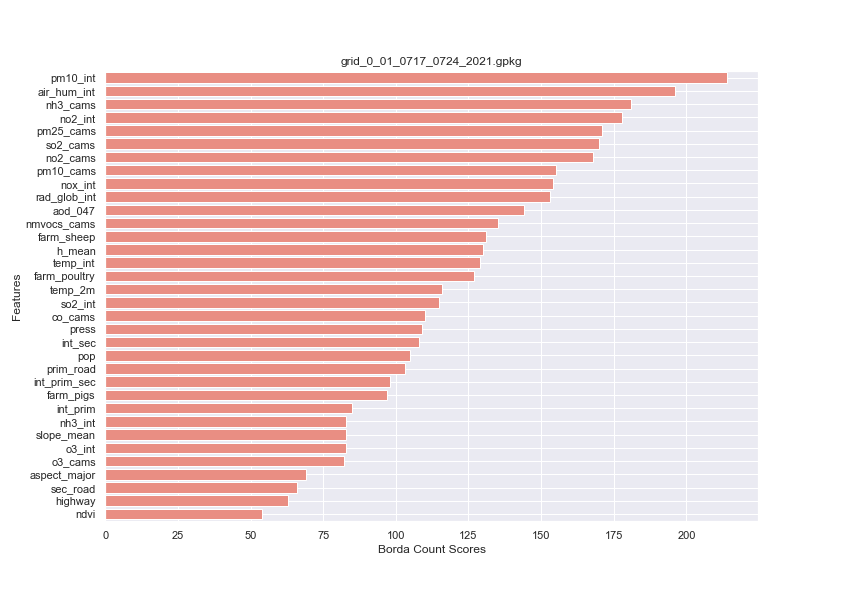
\includegraphics[width=.9\textwidth]{images/fs_results/pm25/001/montains/grid_0_01_0717_0724_2021.png}
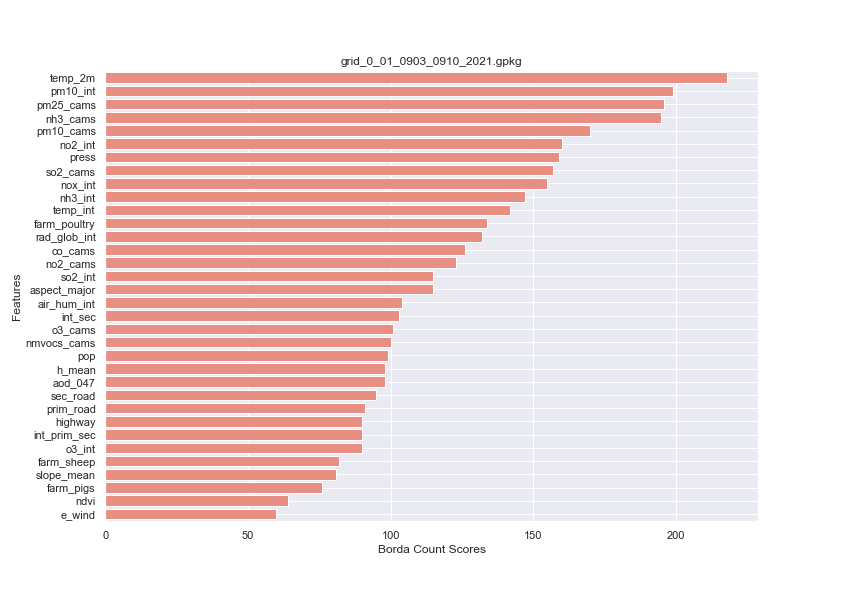
\includegraphics[width=.9\textwidth]{images/fs_results/pm25/001/montains/grid_0_01_0903_0910_2021.png}
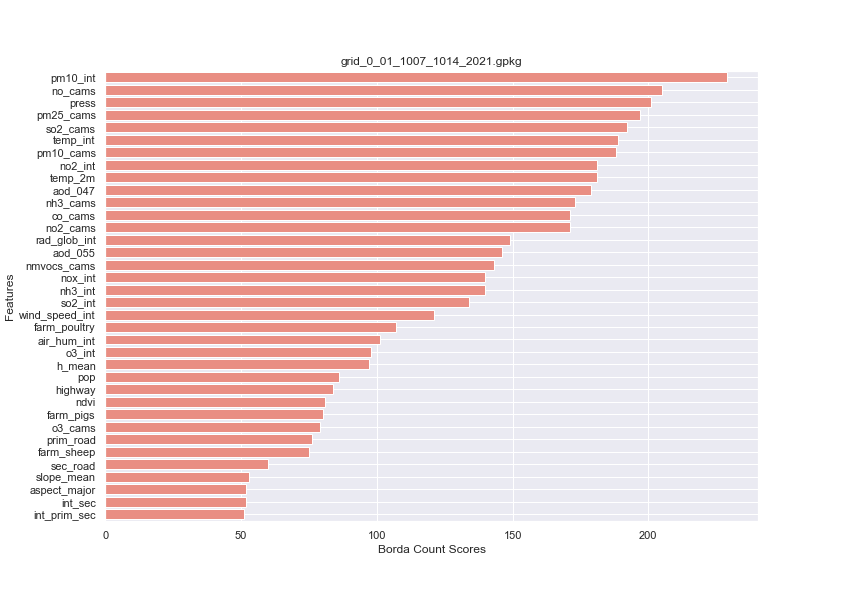
\includegraphics[width=.9\textwidth]{images/fs_results/pm25/001/montains/grid_0_01_1007_1014_2021.png}
\pagebreak
\subsubsection{Excluding mountains}
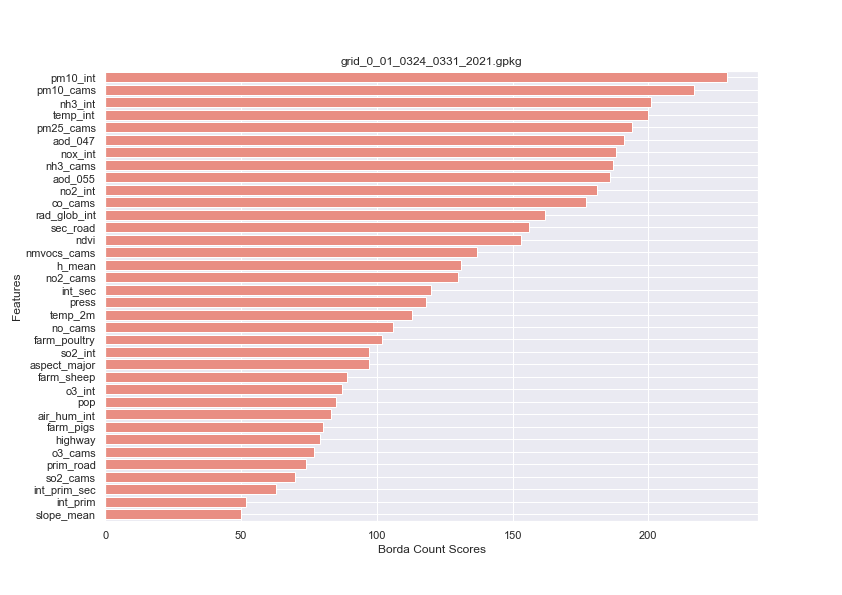
\includegraphics[width=.9\textwidth]{images/fs_results/pm25/001/no_montains/grid_0_01_0324_0331_2021.png}
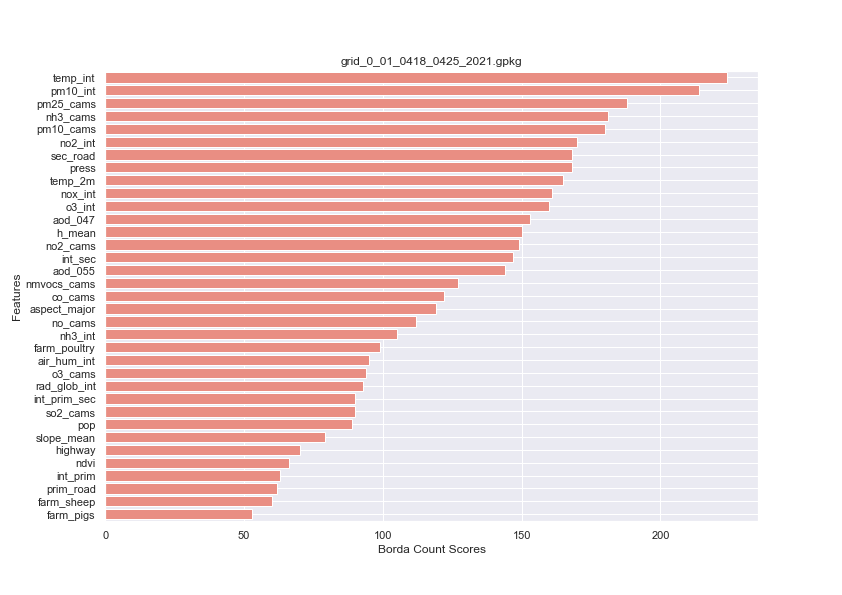
\includegraphics[width=.9\textwidth]{images/fs_results/pm25/001/no_montains/grid_0_01_0418_0425_2021.png}
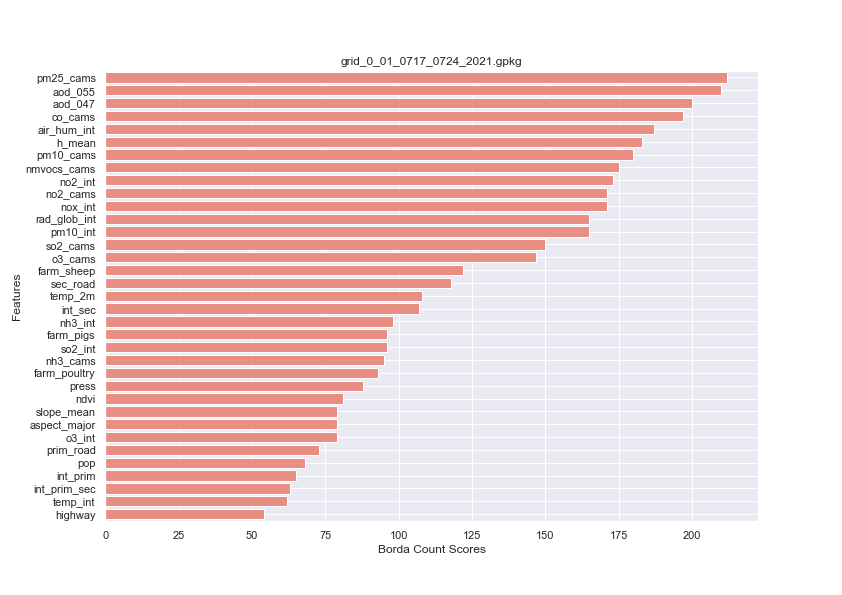
\includegraphics[width=.9\textwidth]{images/fs_results/pm25/001/no_montains/grid_0_01_0717_0724_2021.png}
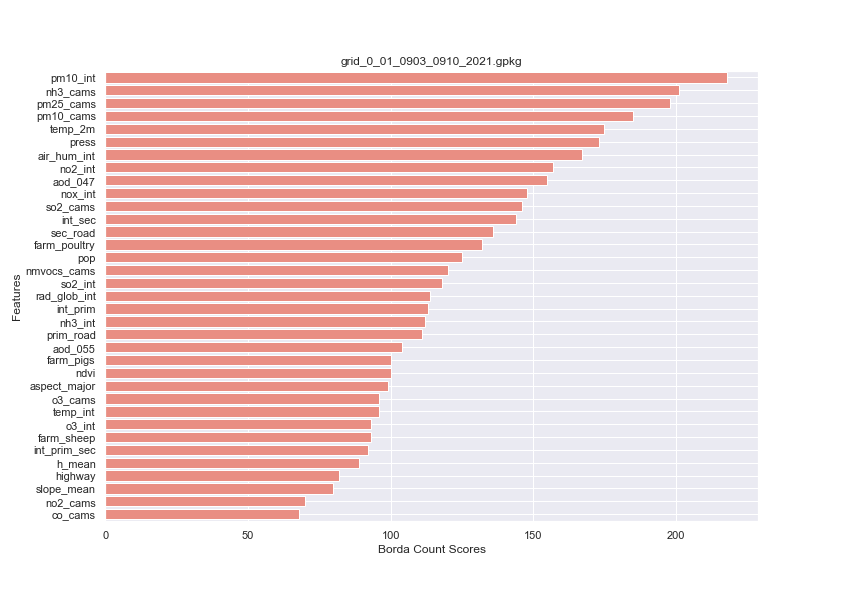
\includegraphics[width=.9\textwidth]{images/fs_results/pm25/001/no_montains/grid_0_01_0903_0910_2021.png}
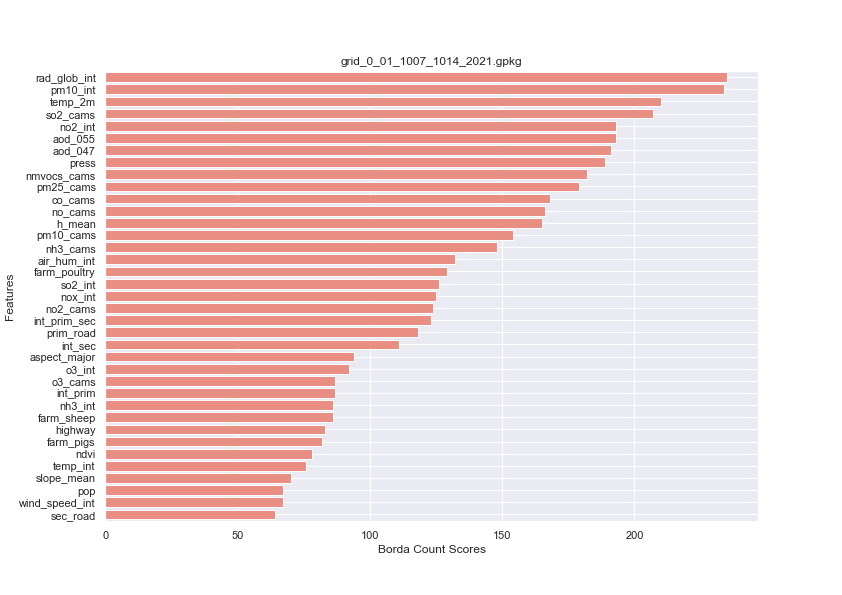
\includegraphics[width=.9\textwidth]{images/fs_results/pm25/001/no_montains/grid_0_01_1007_1014_2021.png}
\subsection{Target variable = 'pm25\_st' \& resolution = 0.1°}
\subsubsection{Including mountains}
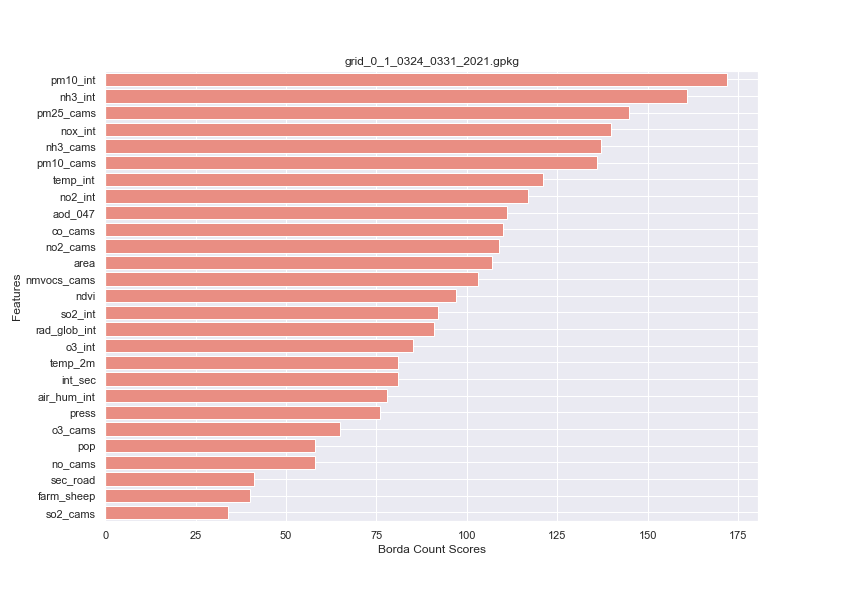
\includegraphics[width=0.9\textwidth]{images/fs_results/pm25/01/montains/grid_0_1_0324_0331_2021.png}
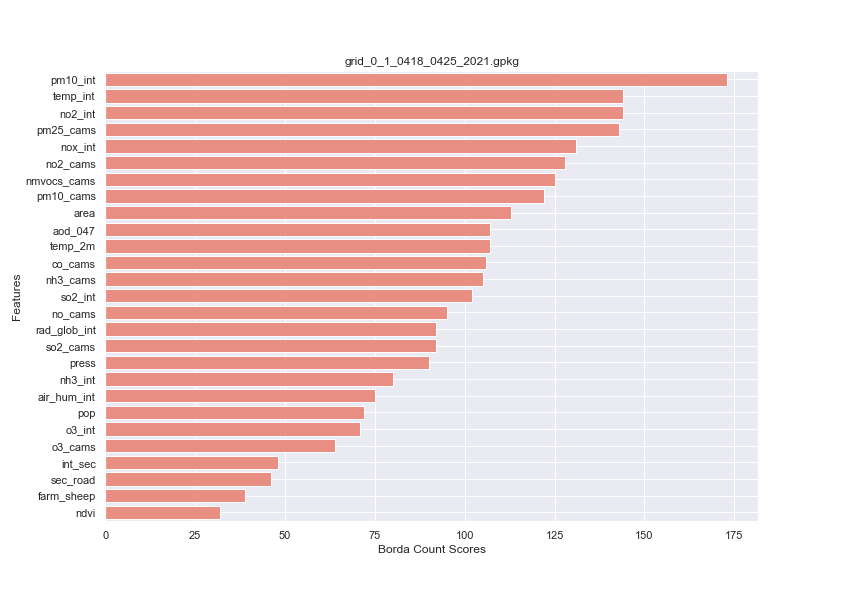
\includegraphics[width=0.9\textwidth]{images/fs_results/pm25/01/montains/grid_0_1_0418_0425_2021.png}
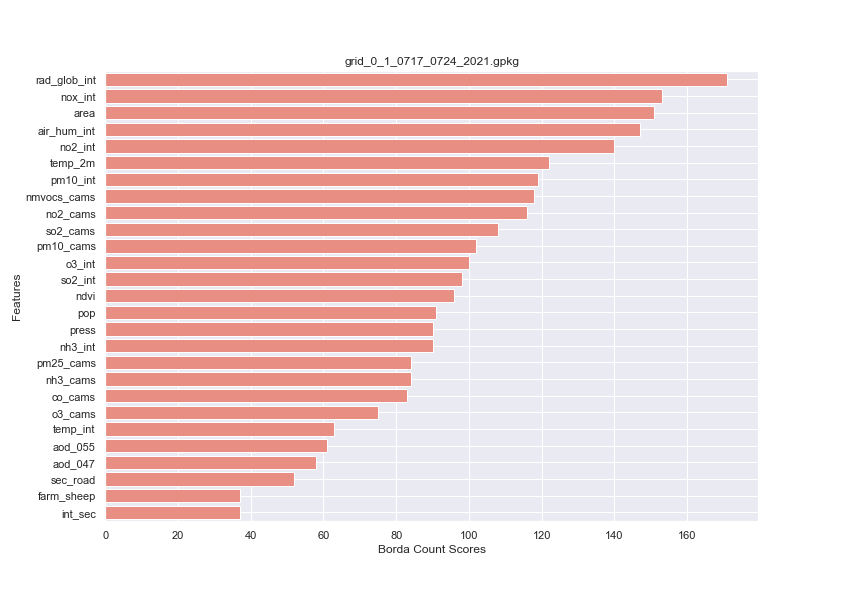
\includegraphics[width=.9\textwidth]{images/fs_results/pm25/01/montains/grid_0_1_0717_0724_2021.png}
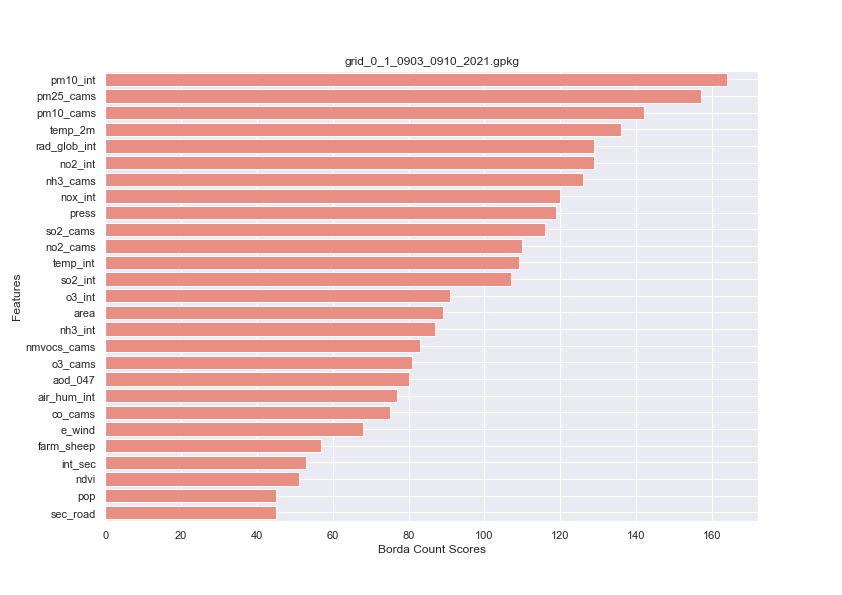
\includegraphics[width=.9\textwidth]{images/fs_results/pm25/01/montains/grid_0_1_0903_0910_2021.png}
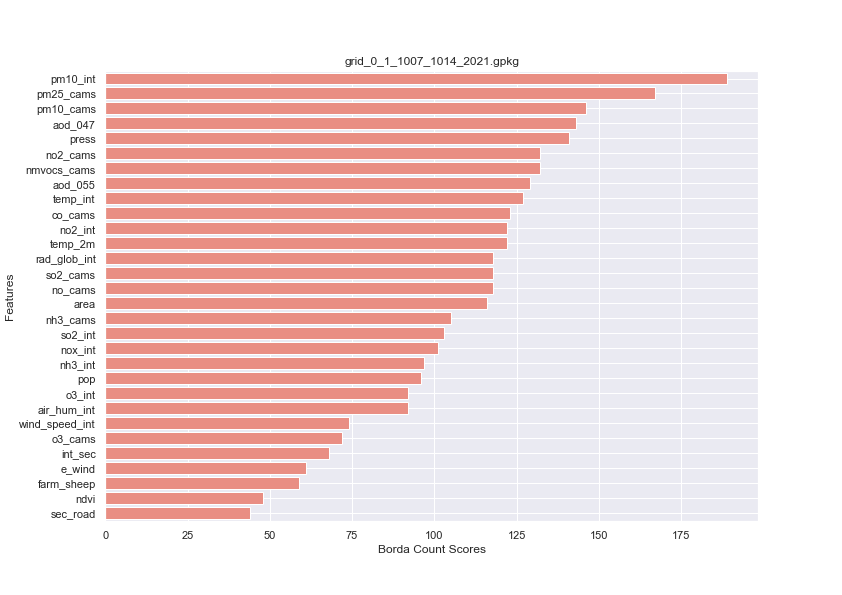
\includegraphics[width=.9\textwidth]{images/fs_results/pm25/01/montains/grid_0_1_1007_1014_2021.png}
\pagebreak
\subsubsection{Excluding mountains}
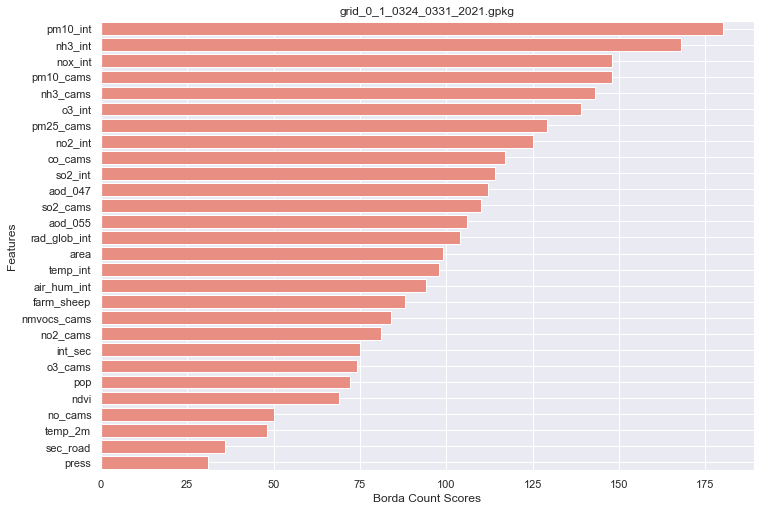
\includegraphics[width=.9\textwidth]{images/fs_results/pm25/01/no_montains/grid_0_1_0324_0331_2021.png}
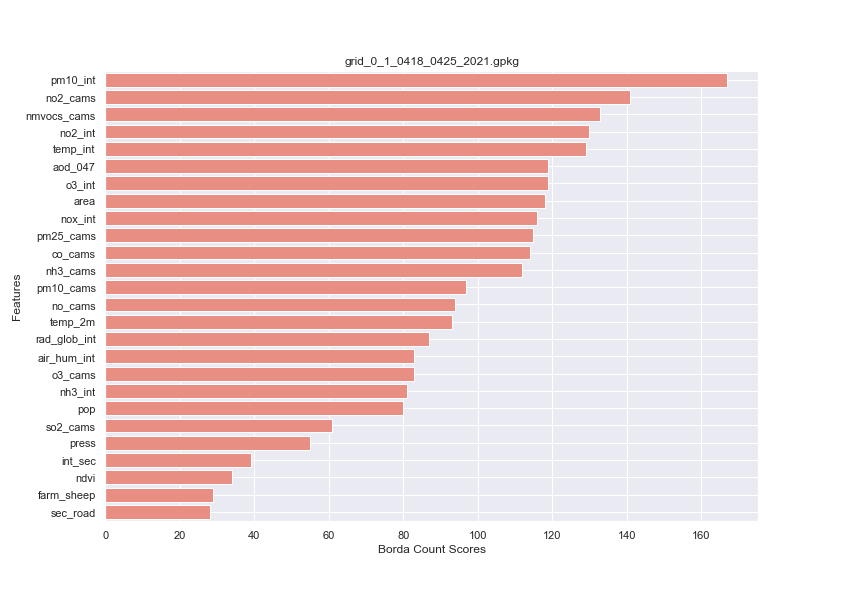
\includegraphics[width=.9\textwidth]{images/fs_results/pm25/01/no_montains/grid_0_1_0418_0425_2021.png}
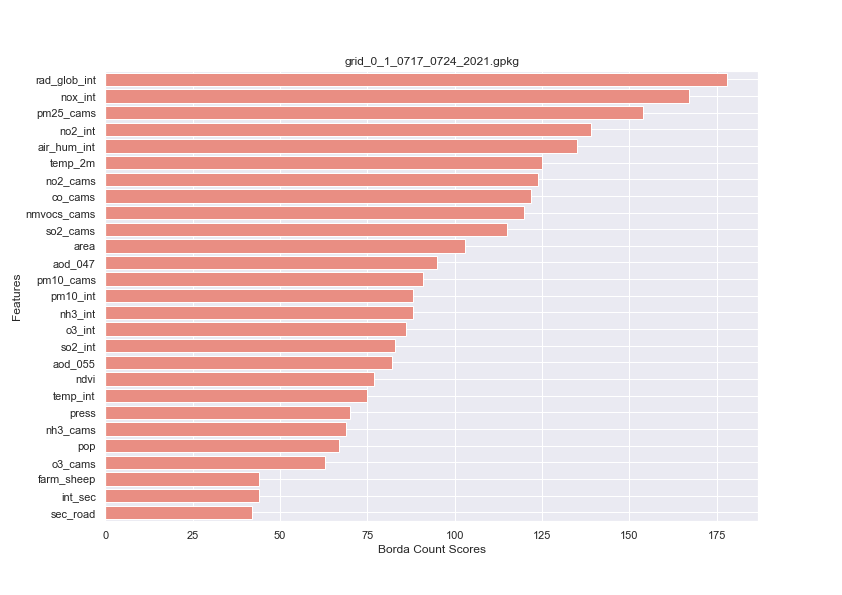
\includegraphics[width=.9\textwidth]{images/fs_results/pm25/01/no_montains/grid_0_1_0717_0724_2021.png}
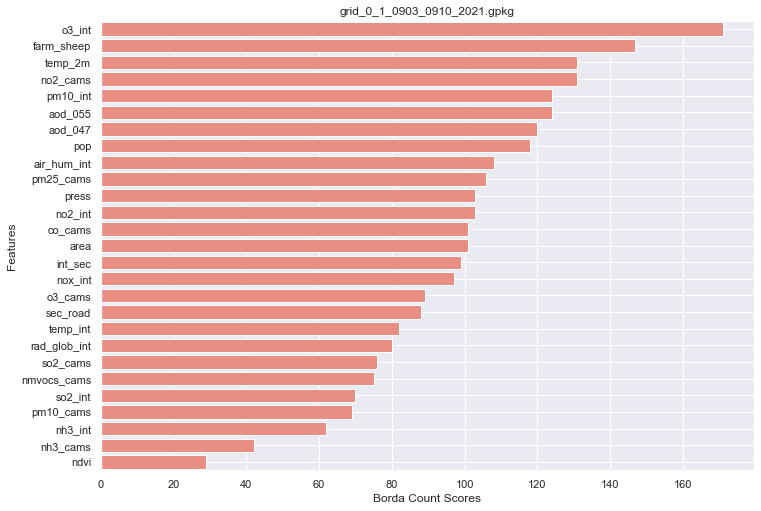
\includegraphics[width=.9\textwidth]{images/fs_results/pm25/01/no_montains/grid_0_1_0903_0910_2021.png}
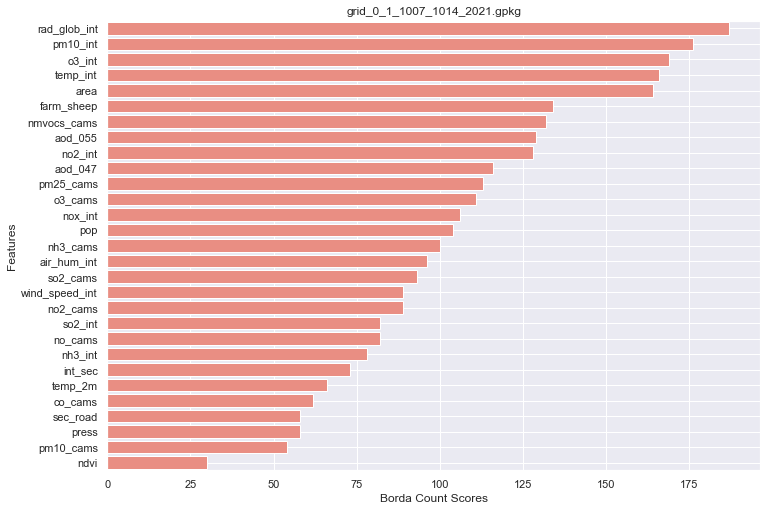
\includegraphics[width=.9\textwidth]{images/fs_results/pm25/01/no_montains/grid_0_1_1007_1014_2021.png}

\begin{comment}
\subsection{Target variable = 'nh3\_st' \& resolution = 0.01°}
\centering
\subsubsection{Including mountains}
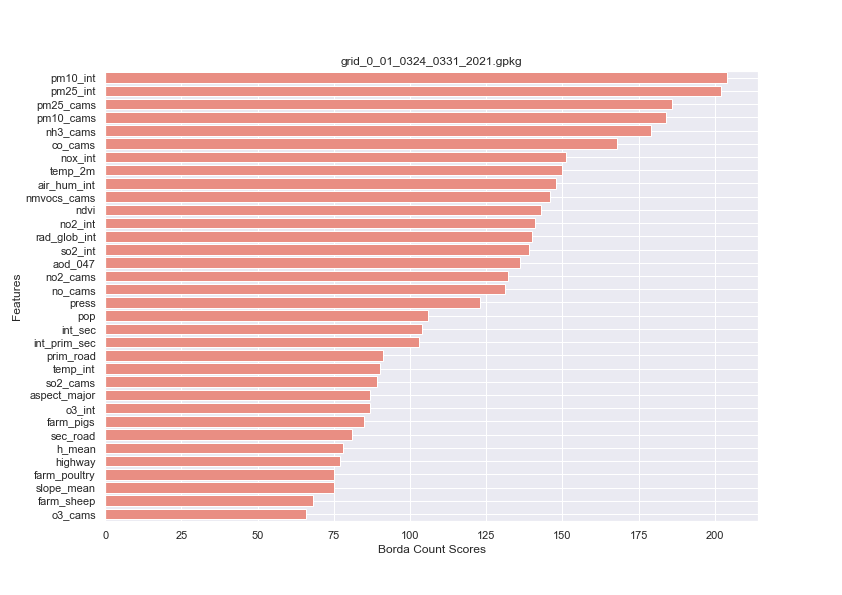
\includegraphics[width=0.9\textwidth]{images/fs_results/nh3/001/montains/grid_0_01_0324_0331_2021.png}
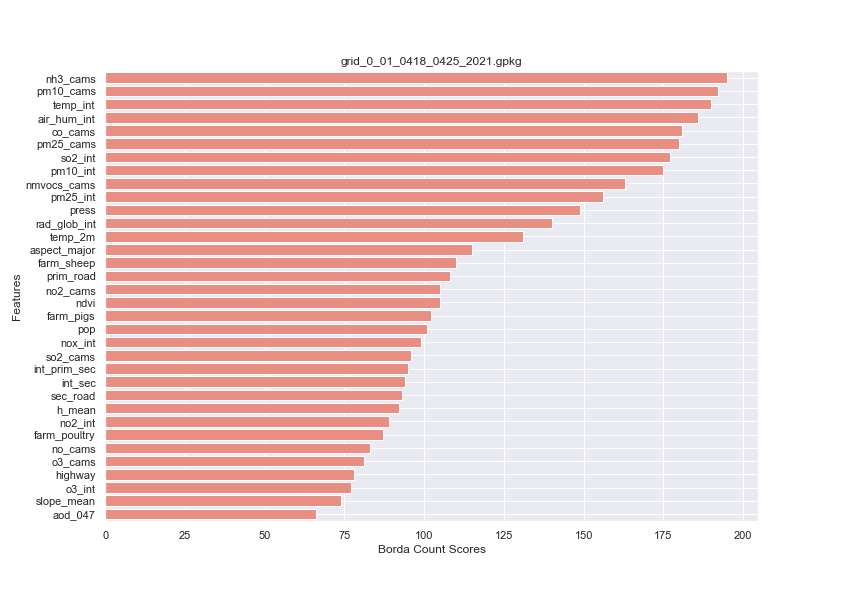
\includegraphics[width=0.9\textwidth]{images/fs_results/nh3/001/montains/grid_0_01_0418_0425_2021.png}
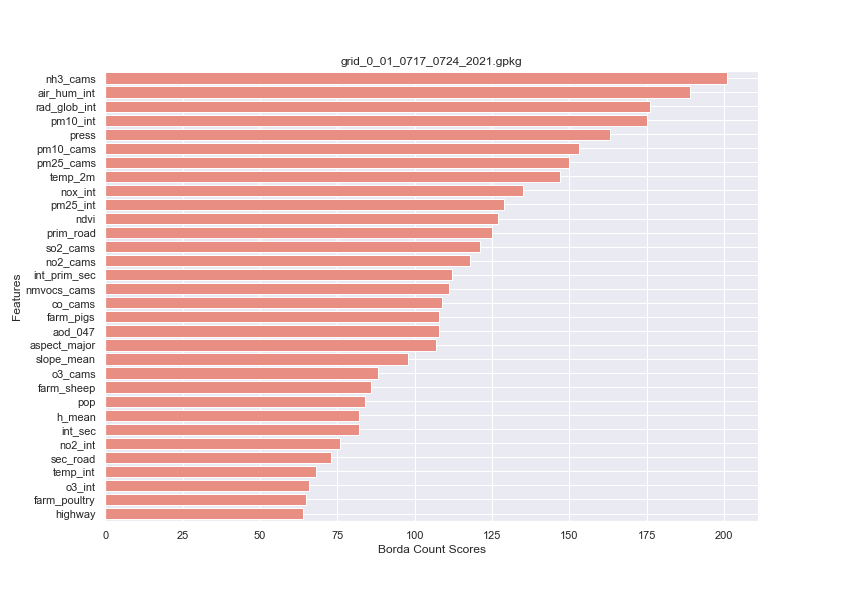
\includegraphics[width=.9\textwidth]{images/fs_results/nh3/001/montains/grid_0_01_0717_0724_2021.png}
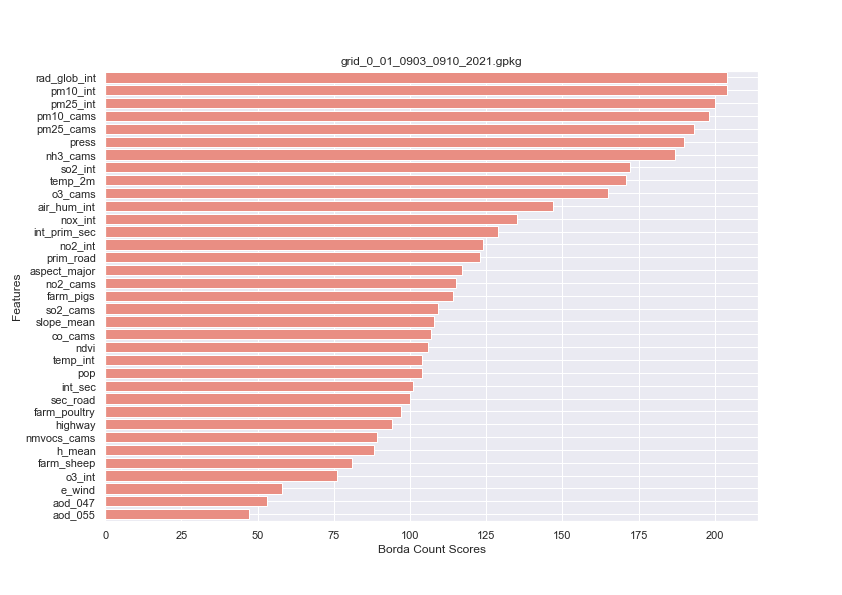
\includegraphics[width=.9\textwidth]{images/fs_results/nh3/001/montains/grid_0_01_0903_0910_2021.png}
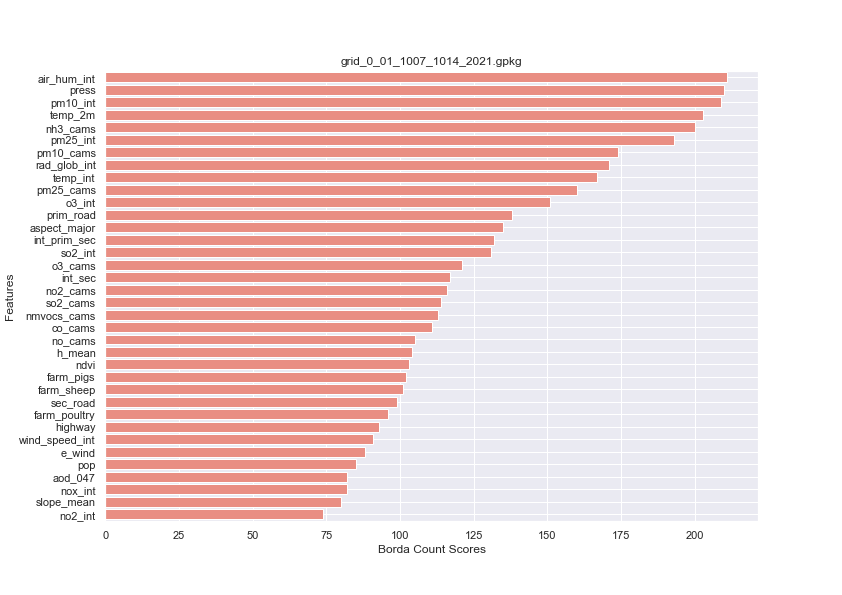
\includegraphics[width=.9\textwidth]{images/fs_results/nh3/001/montains/grid_0_01_1007_1014_2021.png}
\pagebreak
\subsubsection{Excluding mountains}
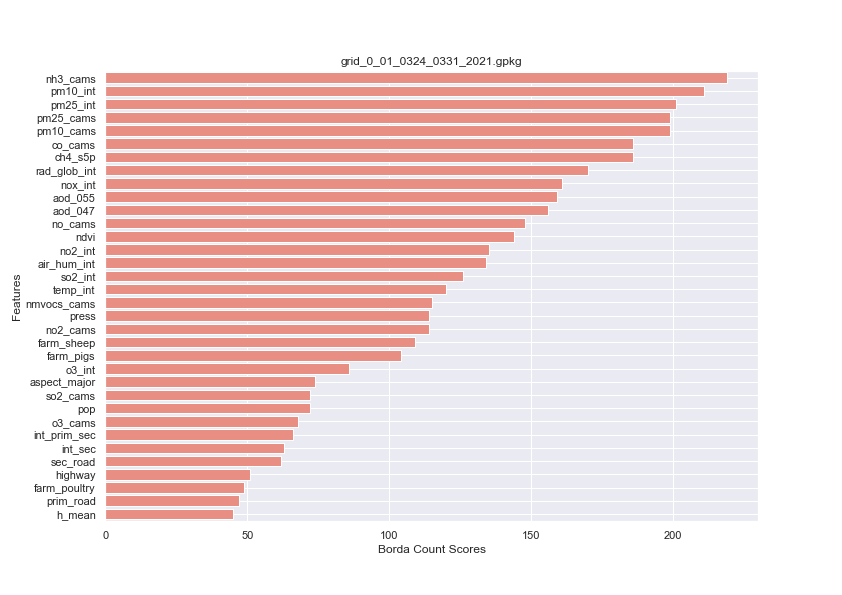
\includegraphics[width=.9\textwidth]{images/fs_results/nh3/001/no_montains/grid_0_01_0324_0331_2021.png}
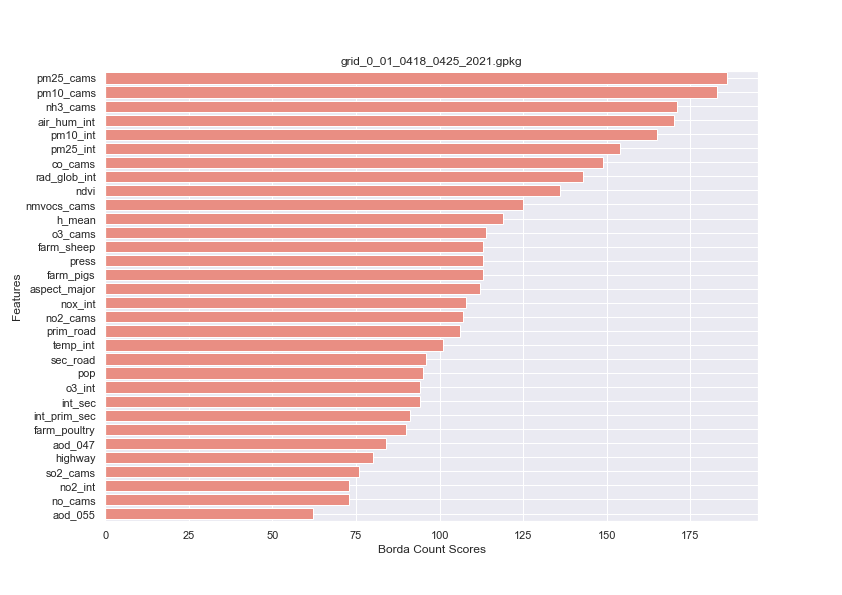
\includegraphics[width=.9\textwidth]{images/fs_results/nh3/001/no_montains/grid_0_01_0418_0425_2021.png}
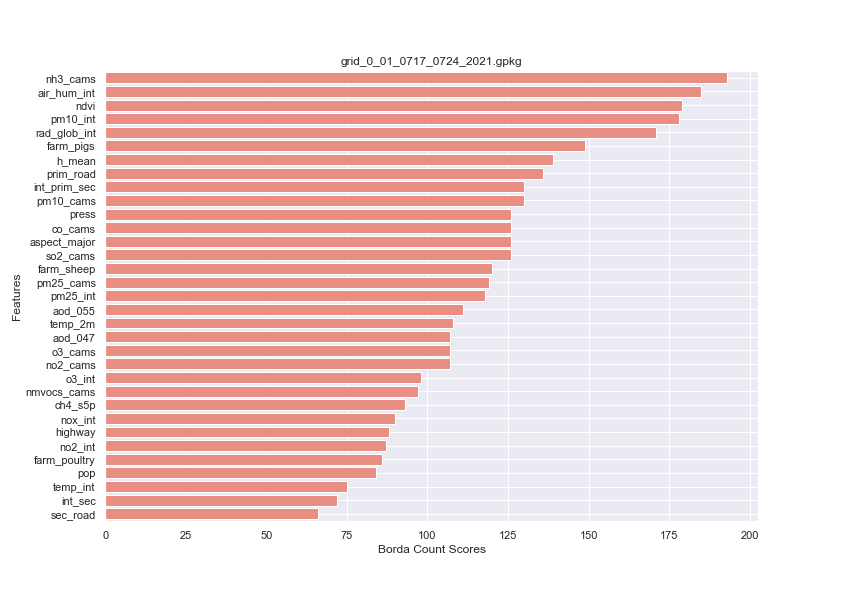
\includegraphics[width=.9\textwidth]{images/fs_results/nh3/001/no_montains/grid_0_01_0717_0724_2021.png}
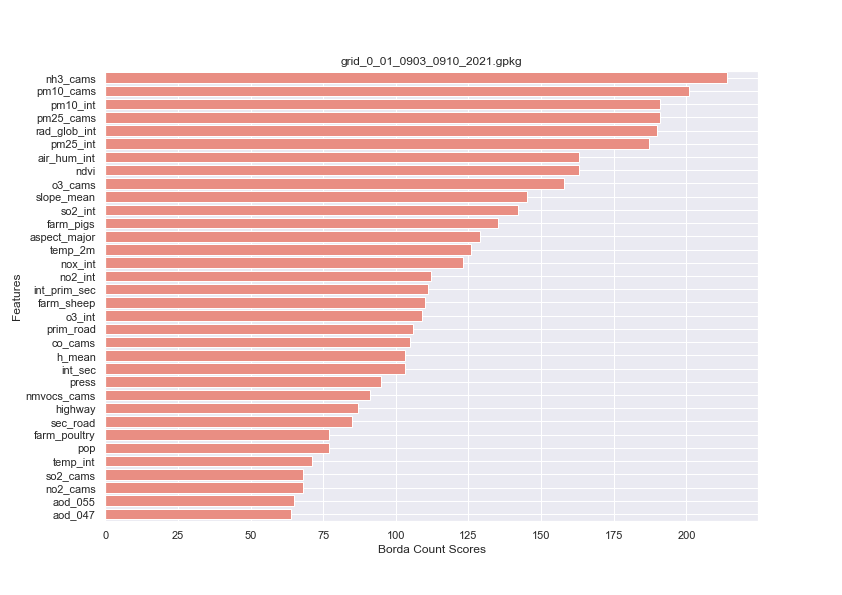
\includegraphics[width=.9\textwidth]{images/fs_results/nh3/001/no_montains/grid_0_01_0903_0910_2021.png}
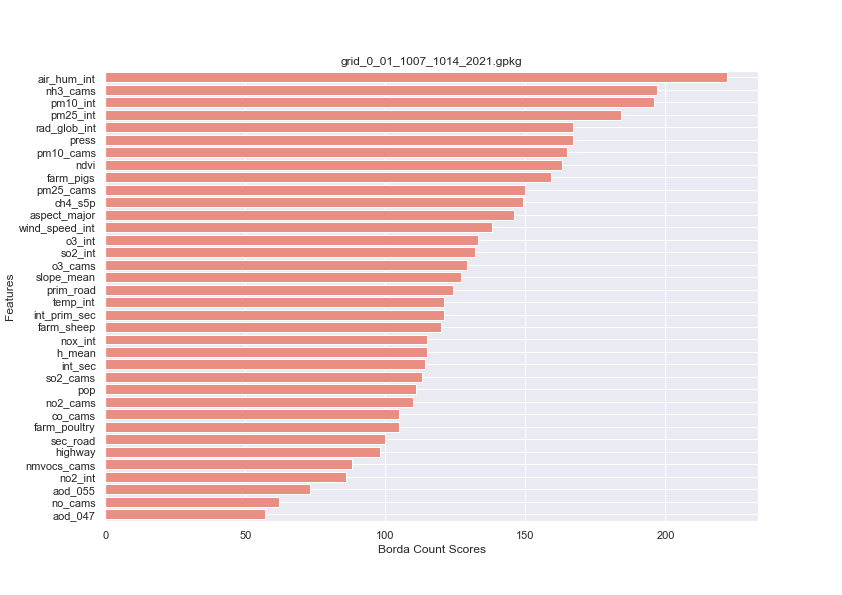
\includegraphics[width=.9\textwidth]{images/fs_results/nh3/001/no_montains/grid_0_01_1007_1014_2021.png}
\end{comment}

\subsection{Target variable = 'nh3\_st' \& resolution = 0.1°}
\subsubsection{Including mountains}
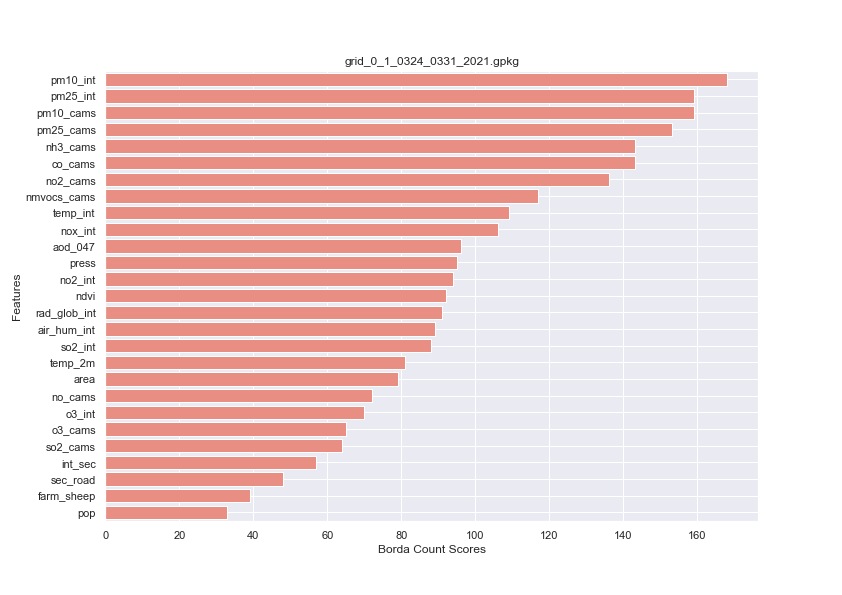
\includegraphics[width=0.9\textwidth]{images/fs_results/nh3/01/montains/grid_0_1_0324_0331_2021.png}
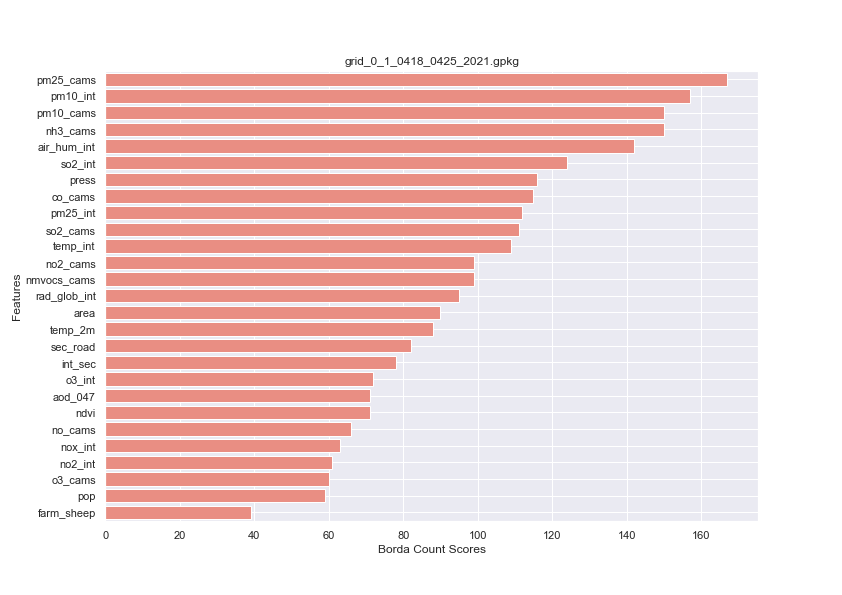
\includegraphics[width=0.9\textwidth]{images/fs_results/nh3/01/montains/grid_0_1_0418_0425_2021.png}
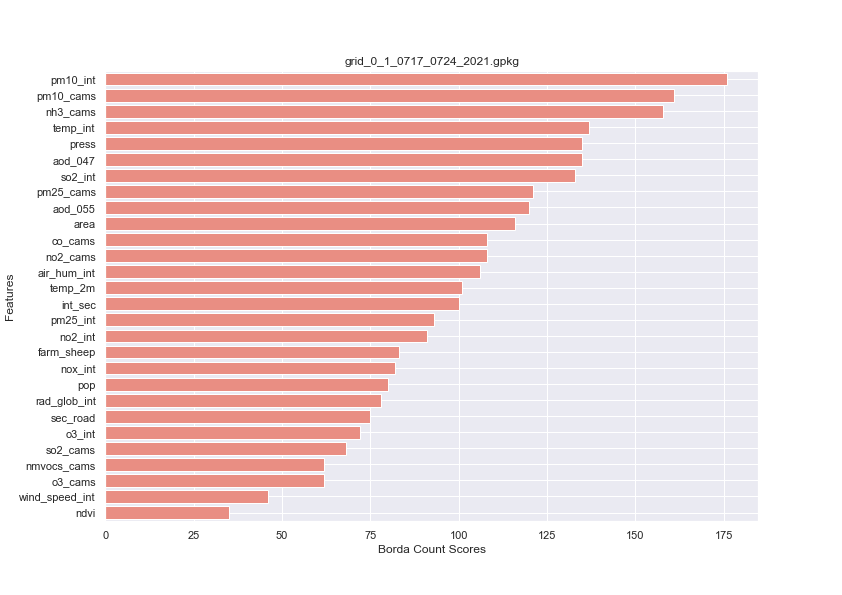
\includegraphics[width=.9\textwidth]{images/fs_results/nh3/01/montains/grid_0_1_0717_0724_2021.png}
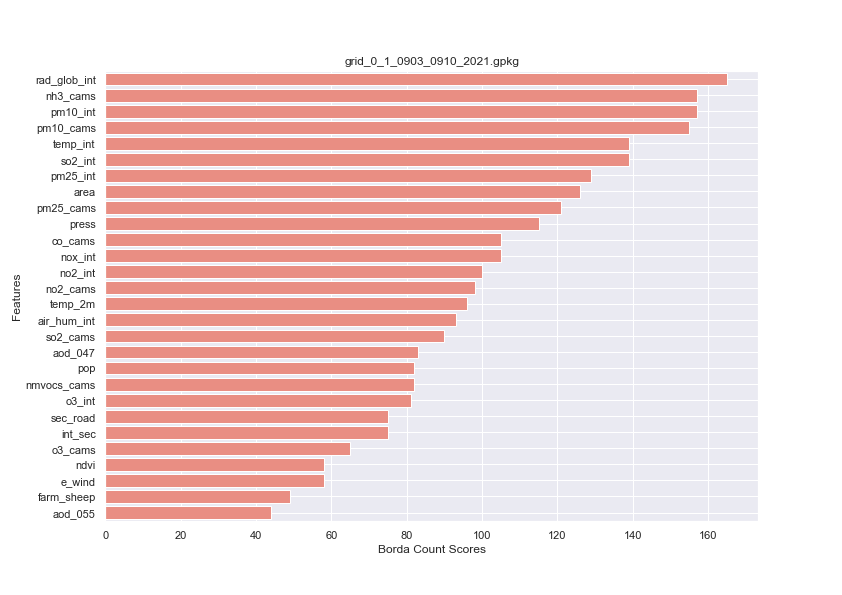
\includegraphics[width=.9\textwidth]{images/fs_results/nh3/01/montains/grid_0_1_0903_0910_2021.png}
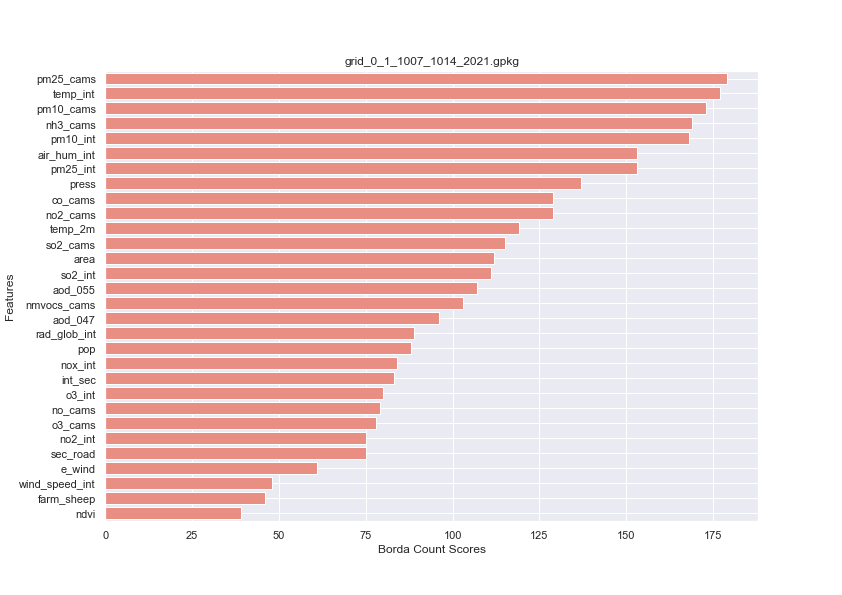
\includegraphics[width=.9\textwidth]{images/fs_results/nh3/01/montains/grid_0_1_1007_1014_2021.png}
\pagebreak
\subsubsection{Excluding mountains}
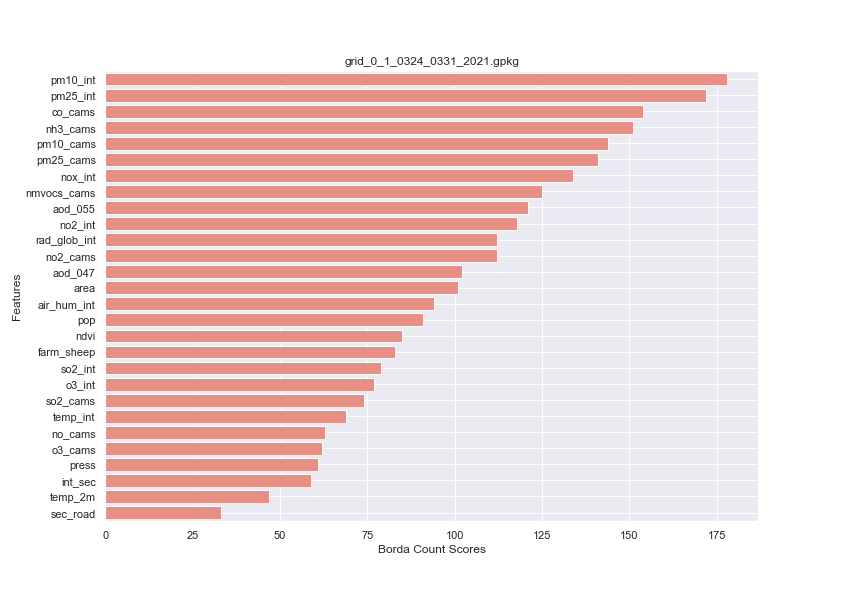
\includegraphics[width=.9\textwidth]{images/fs_results/nh3/01/no_montains/grid_0_1_0324_0331_2021.png}
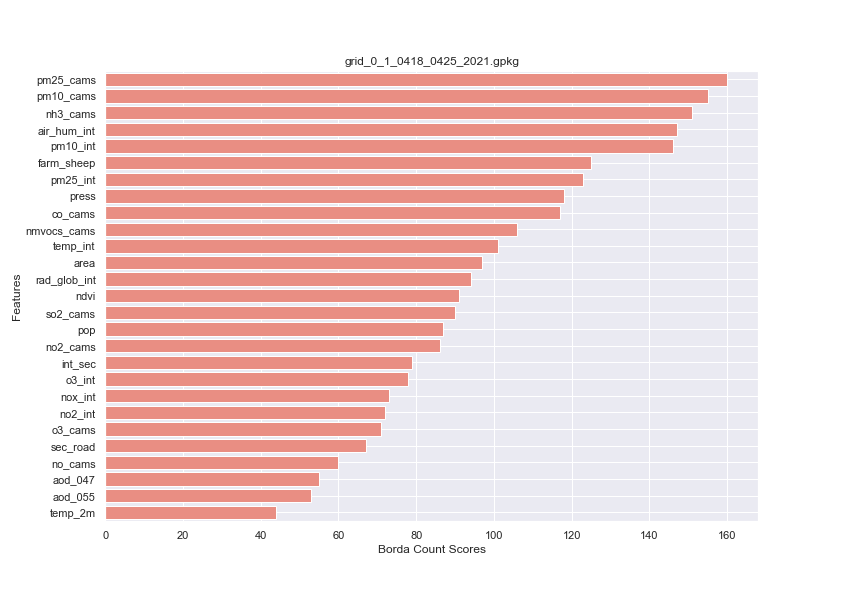
\includegraphics[width=.9\textwidth]{images/fs_results/nh3/01/no_montains/grid_0_1_0418_0425_2021.png}
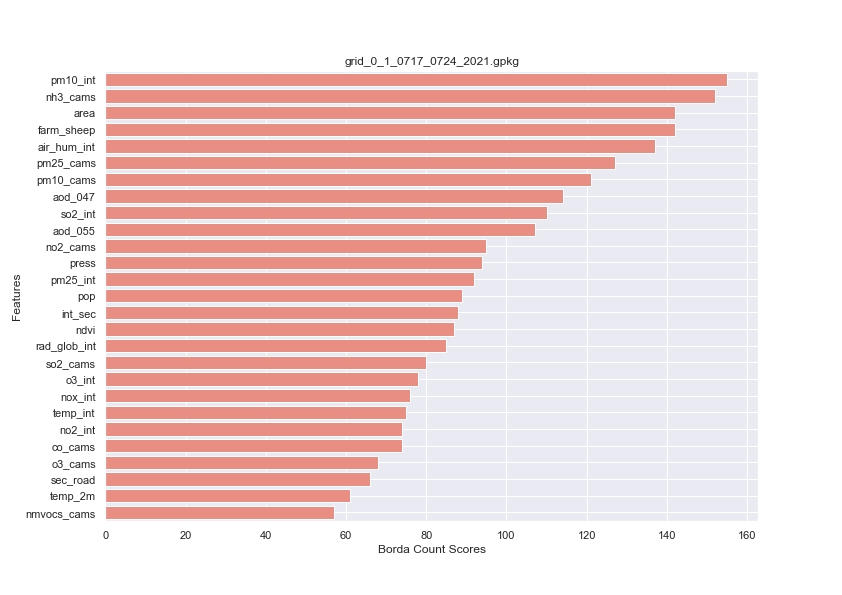
\includegraphics[width=.9\textwidth]{images/fs_results/nh3/01/no_montains/grid_0_1_0717_0724_2021.png}
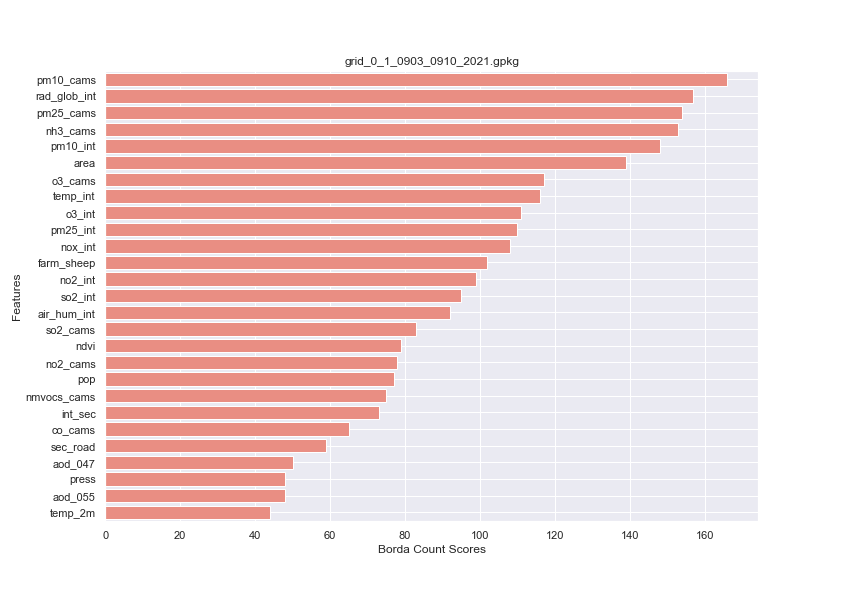
\includegraphics[width=.9\textwidth]{images/fs_results/nh3/01/no_montains/grid_0_1_0903_0910_2021.png}
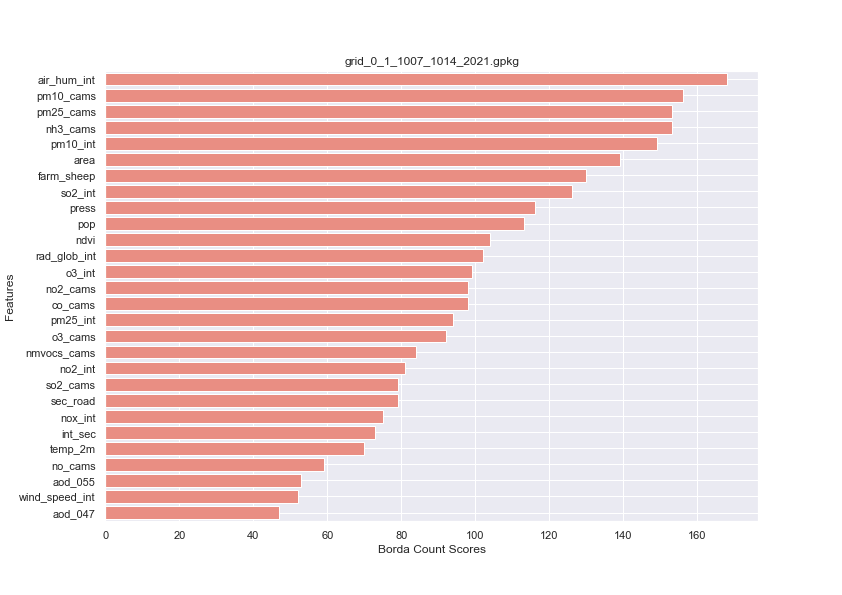
\includegraphics[width=.9\textwidth]{images/fs_results/nh3/01/no_montains/grid_0_1_1007_1014_2021.png}




\subsection{Interpretation of FS results}
\section{Data Modelling}
In this section, I illustrate the models used in order to estimate the target variable. For doing that 2 ML model were implemented:

\subsubsection{Neural Network with Keras}
The neural network was formed by 3 layers
\subsubsection{Random Forest Regressor}

\subsection{Results}
\subsection{Interpretation}

https://www.sciencedirect.com/topics/agricultural-and-biological-sciences/agricultural-pollution 
https://pure.iiasa.ac.at/id/eprint/14769/1/Reduction%20of%20NH3%20emissions%20from%20agriculture%20in%20the%20Hai%20River%20Basin%20in%20China.pdf

https://towardsdatascience.com/batch-mini-batch-stochastic-gradient-descent-7a62ecba642a